Whereas, people have have often tried to categorized objects as GCs by making
cuts along half-light radius, density, and surface brightness profile, in fact
many objects which are generally thought of as GCs don't cleanly fit into these
cuts. Consequently, \citet{Carretta2010} proposed a definition of GC based on
observed chemical inhomogeneities in their stellar populations. The modern
understanding of GCs then is not simply one of a dense cluster of stars which
may have chemical inhomogeneities and multiple populations; rather, it is one
where those chemical inhomogeneities and multiple populations themselves are
the defining element of a GC.

Variations in observed abundances were initially attributed to evolutionary
mixing \citep{Denisenkov1990}. However, enhanced abundances are still observed
in scarcely evolved main sequence stars, ruling out evolutionary mixing as the
primary mechanism \citep{Gratton2004,Briley2004}. Moreover, mixing of a degree
high enough to explain the observed anomaly in cyanogen abundances would result
in extended lifetimes and a broadened main sequence turn off region in the CMD
of ancient GCs, which is not observationally supported. More recently,
precision Hubble photometry revealed that almost every cluster in orbit of the
milky way comprises multiple main sequences \citep{Piotto2007, Roh2011,
Milone2012} (MP) as opposed to a single stellar population (SP).

Due to the relatively high and tight temperature range of partial ionization
for helium it cannot be observed in globular clusters; consequently, the
evidence for these enhanced helium abundances originates from comparison of
theoretical stellar isochrones to the observed color magnitude diagrams of
globular clusters. None of the isochrones used to date in these comparison have
been generated from models with self consistent chemistries. 

\subsection{Population Opacities}
Given the relative historic difficulty in generating new opacity tables,
stellar models have tended to use opacity tables whos range of compositions is
derived from simple rescaling of the some solar composition. Here we use our
OPLIB web scraper to generate opacity tables with compositions specific to each
population in NGC 2808.

These population have been studied in depth by Feiden and their chemical
compositions were determined in \citet{Milone2015} (see Table 2 in that paper).
While we cannot currently make fully self-consistent models due to still
ongoing atmospheric modeling, we can make a first pass investigation of the
affect of OPLIB opacities (Figure \ref{fig:NGC2808ISO}). Note how the models
generated using OPLIB opacity tables have a systematically lower luminosity.
Recall, that this is consistent with the overall lower opacities of the OPLIB
tables.

\begin{figure}
	\centering
	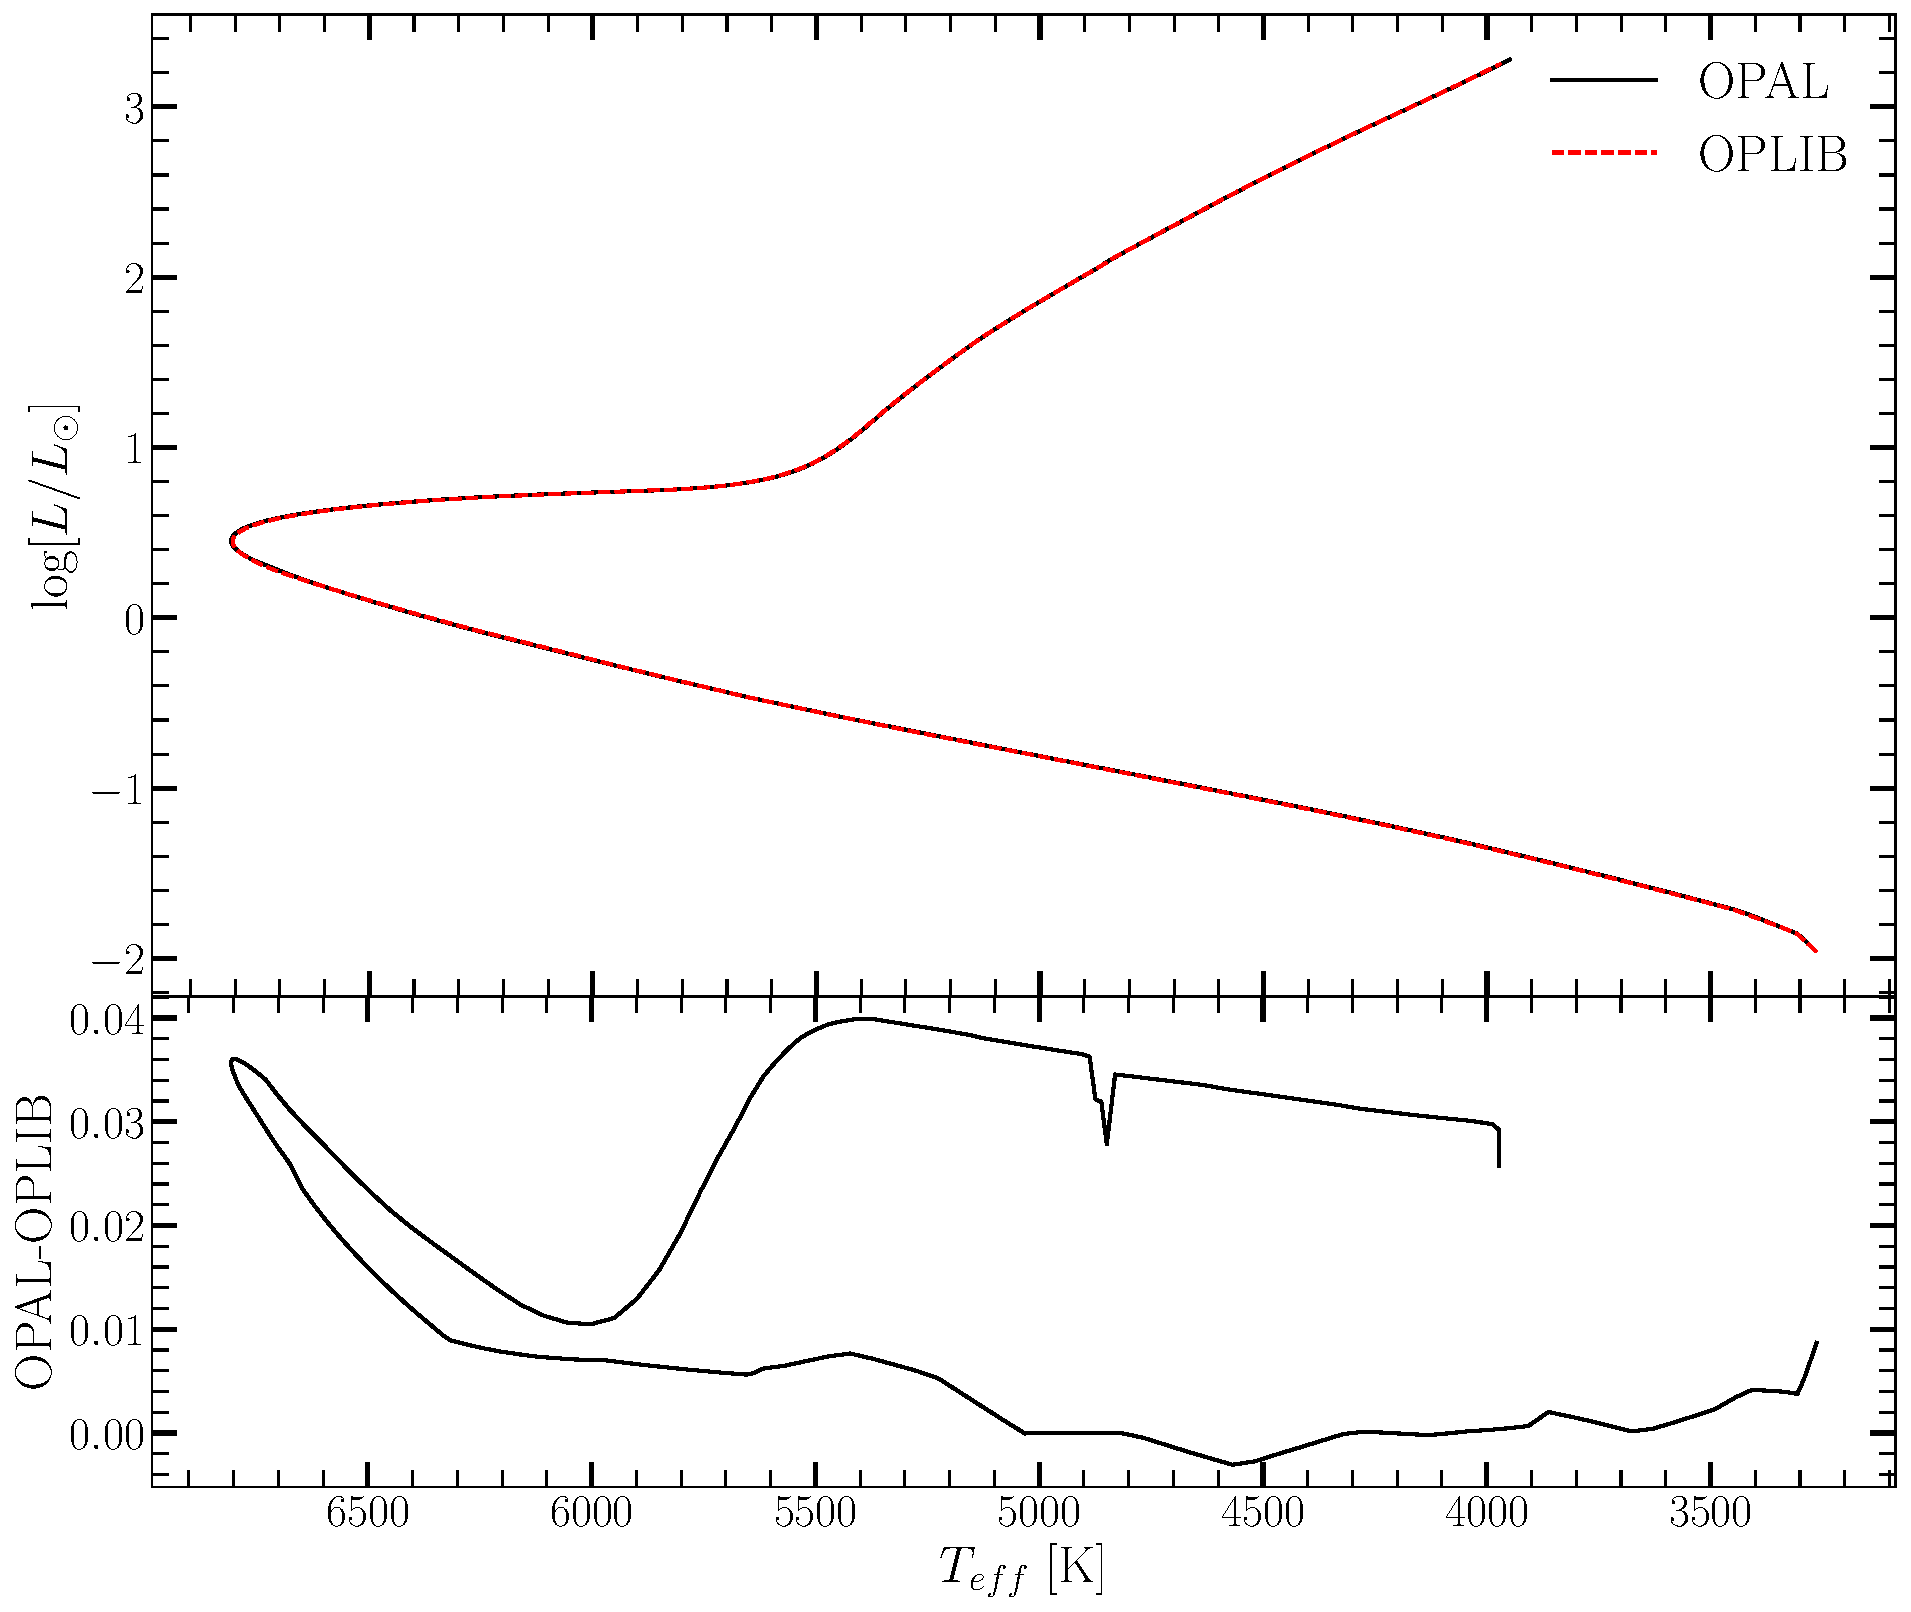
\includegraphics[width=0.45\textwidth]{src/Figures/033ZIsosOPALOPLIB.pdf}
	\caption{10 Gyr \& Y=0.33 isochrones for models generated with OPAL and
	OPLIB opacities tables (top). Residuals between isochrones (bottom).}
	\label{fig:NGC2808ISO}
\end{figure}

\subsection{Additional Consistency}
The lack of self consistency presents problems at other stages of stellar
evolution codes. Perhaps most importantly, where the interior of a stellar
model meets the atmosphere. Atmospheric models such as a grey
\citep{Eddington1916}, Krishna Swamy \citep{Krishna1966}, or Phoenix
\citep{Husser2013} model atmosphere provide one pressure boundary conditions to
solve the two-point boundary value problem that is the equations of stellar
structure. Once again however, models tend to use atmospheres with non
consistent chemistries. Therefore, one key element of NGC 2808 modeling is the
incorporation of new atmospheric models, generated from the MARCS grid of model
atmospheres \citep{Plez2008}, which match interior elemental abundances.
Members of our collaboration are currently working on such atmospheric
modeling.

Finally, The isochrones used to infer the degree of helium enhancements assume
that convection operates in the same manner in metal-poor stars as it does in
the Sun. However, observations from \textit{Kepler} of metal-poor red giants
\citep{Bonaca2012, tayar2017correlation}, in concert with interferometric
radius determination of the metal-poor sub-giant HD 140283
\citep{creevey2015benchmark}, have shown that the efficiency of convection
changes with iron content. We will additionally modify DSEP to capture this
variation in convective efficiency. While we wait for atmospheric modeling to
be completed it makes sense to investigate other locations where opacity
differences on the order of 5\% may affect results."s
